\chapter{Cyclopts HDF5 Database Layout}\label{app:hdf5}

This appendix details the exact database layout used by Cyclopts for the
\texttt{ExchangeFamily}, \texttt{StructuredRequest} species, and
\texttt{StructuredSupply} species.

\section{Parameter Space}

Both front-end and back-end species record the state of every point in a given
parameter space in a data set called \code{/Species/<species type>/Points},
where \code{<species type>} is either \code{StructuredRequest} or
\code{StructuredSupply}. Each point incorporates both fundamental and instance
parameters as described in \S \ref{method:setup}. The tables associated with
parameter spaces are described in Tables
\ref{tbl:/Species/StructuredRequest/Points}-\ref{tbl:/Species/StructuredSupply/Points}.

\begin{table}[h!]
\centering
\caption{\label{tbl:/Species/StructuredRequest/Points}
Data-type description of the \lstinline[basicstyle=\ttfamily\color{black}]|/Species/StructuredRequest/Points| dataset.}
\begin{tabularx}{\columnwidth-10pt}{|c|c|X|} % line wraps second column if too long
\hline
\textbf{Name} & \textbf{Data Type} & \textbf{Description}       \\ \hline
paramid & 16-character string & The hex value of a UUID for a point in parameter space. \\ \hline
family & 30-character string & A description of the problem family \\ \hline
f\_fc & 1-byte integer & As described in \S \ref{method:setup} \\ \hline
f\_loc & 1-byte integer & As described in \S \ref{method:setup} \\ \hline
f\_mox & 4-byte float & As described in \S \ref{method:setup} \\ \hline
f\_rxtr & 1-byte integer & As described in \S \ref{method:setup} \\ \hline
n\_reg & 4-byte unsigned integer & As described in \S \ref{method:setup} \\ \hline
n\_rxtr & 4-byte unsigned integer & As described in \S \ref{method:setup} \\ \hline
r\_inv\_proc & 4-byte float & As described in \S \ref{method:setup} \\ \hline
r\_l\_c & 4-byte float & As described in \S \ref{method:setup} \\ \hline
r\_s\_mox & 4-byte float & As described in \S \ref{method:setup} \\ \hline
r\_s\_mox\_uox & 4-byte float & As described in \S \ref{method:setup} \\ \hline
r\_s\_th & 4-byte float & As described in \S \ref{method:setup} \\ \hline
r\_s\_thox & 4-byte float & As described in \S \ref{method:setup} \\ \hline
r\_t\_f & 4-byte float & As described in \S \ref{method:setup} \\ \hline
r\_th\_pu & 4-byte float & As described in \S \ref{method:setup} \\ \hline
seed & 8-byte integer & The random seed used to generate an instance. \\ \hline
\end{tabularx}
\end{table}


\begin{table}[h!]
\centering
\caption{\label{tbl:/Species/StructuredSupply/Points}
Datatype description of the \lstinline[basicstyle=\ttfamily\color{black}]|/Species/StructuredSupply/Points| dataset.}
\begin{tabularx}{\columnwidth-10pt}{|c|c|X|} % line wraps second column if too long
\hline
\textbf{Name} & \textbf{Data Type} & \textbf{Description}       \\ \hline
paramid & 16-character string & The hex value of a UUID for a point in parameter space. \\ \hline
family & 30-character string & A description of the problem family \\ \hline
d\_f\_mox & 4-length array of 8-byte floats & As described in \S \ref{method:setup} \\ \hline
d\_f\_thox & 4-length array of 8-byte floats & As described in \S \ref{method:setup} \\ \hline
d\_th & 3-length array of 8-byte floats & As described in \S \ref{method:setup} \\ \hline
f\_fc & 1-byte integer & As described in \S \ref{method:setup} \\ \hline
f\_loc & 1-byte integer & As described in \S \ref{method:setup} \\ \hline
f\_mox & 4-byte float & As described in \S \ref{method:setup} \\ \hline
f\_rxtr & 1-byte integer & As described in \S \ref{method:setup} \\ \hline
n\_reg & 4-byte unsigned integer & As described in \S \ref{method:setup} \\ \hline
n\_rxtr & 4-byte unsigned integer & As described in \S \ref{method:setup} \\ \hline
r\_inv\_proc & 4-byte float & As described in \S \ref{method:setup} \\ \hline
r\_l\_c & 4-byte float & As described in \S \ref{method:setup} \\ \hline
r\_repo & 4-byte float & As described in \S \ref{method:setup} \\ \hline
r\_s\_mox & 4-byte float & As described in \S \ref{method:setup} \\ \hline
r\_s\_mox\_uox & 4-byte float & As described in \S \ref{method:setup} \\ \hline
r\_s\_th & 4-byte float & As described in \S \ref{method:setup} \\ \hline
r\_s\_thox & 4-byte float & As described in \S \ref{method:setup} \\ \hline
r\_t\_f & 4-byte float & As described in \S \ref{method:setup} \\ \hline
r\_th\_pu & 4-byte float & As described in \S \ref{method:setup} \\ \hline
seed & 8-byte integer & The random seed used to generate an instance. \\ \hline
\end{tabularx}
\end{table}

\section{Problem Instances}

Problem instances are generated by problem species and are executed by problem
families. Accordingly, both species and families can record information about
instances. Front and back-end exchange species each record two types of
information: details about each arc in an instance and a summary of
species-specific information. The exchange family records information regarding
each of the entities that comprise an instance: nodes, groups of nodes (having
been translated from portfolios), and arcs. Further, aggregate summary
information is also recorded. 

\subsection{Exchange Family}

The exchange family records information regarding all major constructs in an
exchange: nodes, groups, and arcs. A summary table is written to
\texttt{/Family/ResourceExchange/ExchangeInstProperties}. Nodes and group data
are recorded in an aggregate dataset located at
\texttt{/Family/ResourceExchange/ExchangeNodes}, node group data is located at
\texttt{/Family/ResourceExchange/ExchangeGroups}, and arc data is collected in
the \texttt{/Family/ResourceExchange/ExchangeArcs} group. A dataset per instance
UUID is used because it has been found to have better performance in the
post-processing phase. A summary of family-specific instance data are detailed in
Tables
\ref{tbl:/Family/ResourceExchange/ExchangeInstProperties}-\ref{tbl:/Family/ResourceExchange/ExchangeArcs}.

\begin{table}[h!]
\centering
\caption{\label{tbl:/Family/ResourceExchange/ExchangeInstProperties}
Datatype description of the \lstinline[basicstyle=\ttfamily\color{black}]|/Family/ResourceExchange/ExchangeInstProperties| dataset.}
\begin{tabularx}{\columnwidth-10pt}{|c|c|X|} % line wraps second column if too long
\hline
\textbf{Name} & \textbf{Data Type} & \textbf{Description}       \\ \hline
paramid & 16-character string & The hex value of a UUID for a point in parameter space. \\ \hline
instid & 16-character string & The hex value of a UUID for an NFCTP graph instance. \\ \hline
species & 30-character string & A description of a problem species. \\ \hline
n\_arcs & 8-byte integer & The number of arcs in an NFCTP instance. \\ \hline
n\_u\_grps & 8-byte integer & The number of supply groups in an NFCTP instance. \\ \hline
n\_v\_grps & 8-byte integer & The number of demand groups in an NFCTP instance. \\ \hline
n\_u\_nodes & 8-byte integer & The number of supply nodes in an NFCTP instance. \\ \hline
n\_v\_nodes & 8-byte integer & The number of demand nodes in an NFCTP instance. \\ \hline
n\_constrs & 8-byte integer & The number of constraints in an NFCTP instance. \\ \hline
excl\_frac & 8-byte float & The fraction of arcs in a NFCTP graph that are exclusive. \\ \hline
\end{tabularx}
\end{table}

\begin{table}[h!]
\centering
\label{tbl:/Family/ResourceExchange/ExchangeNodes}
\caption{Datatype description of the \lstinline[basicstyle=\ttfamily\color{black}]|/Family/ResourceExchange/ExchangeNodes| dataset.}
\begin{tabularx}{\columnwidth-10pt}{|c|c|X|} % line wraps second column if too long
\hline
\textbf{Name} & \textbf{Data Type} & \textbf{Description}       \\ \hline
instid & 16-character string & The hex value of a UUID for an NFCTP graph instance. \\ \hline
id & 8-byte integer & A uniquely identifying value. \\ \hline
gid & 8-byte integer & A unique value identifying an ExchangeGroup \\ \hline
kind & 1-byte integer bitfield & Whether an object is associated with supply or demand. \\ \hline
qty & 8-byte float & A quantity. \\ \hline
excl & 1-byte integer bitfield & Whether or not an arc is exclusive. \\ \hline
excl\_id & 8-byte integer & A unique value identifying the mutually exclusive group an arc belongs to. \\ \hline
\end{tabularx}
\end{table}

\begin{table}[h!]
\centering
\label{tbl:/Family/ResourceExchange/ExchangeGroups}
\caption{Datatype description of the \lstinline[basicstyle=\ttfamily\color{black}]|/Family/ResourceExchange/ExchangeGroups| dataset.}
\begin{tabularx}{\columnwidth-10pt}{|c|c|X|} % line wraps second column if too long
\hline
\textbf{Name} & \textbf{Data Type} & \textbf{Description}       \\ \hline
instid & 16-character string & The hex value of a UUID for an NFCTP graph instance. \\ \hline
id & 8-byte integer & A uniquely identifying value. \\ \hline
kind & 1-byte integer bitfield & Whether an object is associated with supply or demand. \\ \hline
caps & 4-length array of 8-byte floats & Capacity RHS values. \\ \hline
cap\_dirs & 4-length array of 1-byte integer bitfields & Whether a constraint is greater or less-than \\ \hline
qty & 8-byte float & A quantity. \\ \hline
\end{tabularx}
\end{table}

\begin{table}[h!]
\centering
\caption{
\label{tbl:/Family/ResourceExchange/ExchangeArcs}
Datatype description of the \lstinline[basicstyle=\ttfamily\color{black}]|/Family/ResourceExchange/ExchangeArcs/<Instance UUID>| dataset.}
\begin{tabularx}{\columnwidth-10pt}{|c|c|X|} % line wraps second column if too long
\hline
\textbf{Name} & \textbf{Data Type} & \textbf{Description}       \\ \hline
id & 8-byte integer & A uniquely identifying value. \\ \hline
uid & 8-byte integer & Supply node for an arc. \\ \hline
ucaps & 4-length array of 8-byte floats & Capacity coefficients for a supply node. \\ \hline
vid & 8-byte integer & Request node for an arc. \\ \hline
vcaps & 4-length array of 8-byte floats & Capacity coefficients for a request node. \\ \hline
pref & 8-byte float & Preference value of an arc. \\ \hline
\end{tabularx}
\end{table}

\subsection{Exchange Species}

Both exchange species record information about each arc in an exchange
instance. A parent group for arc data is defined under each species group. A
group for each instance, whose name is the hex string of the UUID, is defined
under the associated arc group. Finally, arc information associated with each
instance is stored as a dataset in that instance's group. For example, the arc
data for a given UUID of a front-end exchange is located as a dataset in the
group \texttt{/Species/StructuredRequest/Arcs/<UUID hex>}. Summary information
related to each species is also recorded in a data set for each species type
located in the group \texttt{/Species/<species type>/Summary}. Tables describing
species-specific instance data are detailed in Tables
\ref{tbl:/Species/StructuredRequest/Arcs/id_8017b48888ac424fb991527195a831b6}-\ref{tbl:/Species/StructuredSupply/Summary}.

\begin{table}[h!]
\centering
\caption{\label{tbl:/Species/StructuredRequest/Arcs/id_8017b48888ac424fb991527195a831b6}
Datatype description of the \lstinline[basicstyle=\ttfamily\color{black}]|/Species/<Species Type>/Arcs/<Instance UUID>| dataset.}
\begin{tabularx}{\columnwidth-10pt}{|c|c|X|} % line wraps second column if too long
\hline
\textbf{Name} & \textbf{Data Type} & \textbf{Description}       \\ \hline
arcid & 4-byte unsigned integer & The hex value of a UUID for an arc. \\ \hline
commod & 4-byte unsigned integer & The commodity associated with an arc. \\ \hline
pref\_c & 4-byte float & Commodity-based preference of an arc. \\ \hline
pref\_l & 4-byte float & Location-based preference of an arc. \\ \hline
\end{tabularx}
\end{table}

\begin{table}[h!]
\centering
\label{tbl:/Species/StructuredRequest/Summary}
\caption{Datatype description of the \lstinline[basicstyle=\ttfamily\color{black}]|/Species/StructuredRequest/Summary| dataset.}
\begin{tabularx}{\columnwidth-10pt}{|c|c|X|} % line wraps second column if too long
\hline
\textbf{Name} & \textbf{Data Type} & \textbf{Description}       \\ \hline
paramid & 16-character string & The hex value of a UUID for a point in parameter space. \\ \hline
family & 30-character string & A description of the problem family \\ \hline
n\_r\_th & 4-byte unsigned integer & As described in \S \ref{method:setup} \\ \hline
n\_r\_f\_mox & 4-byte unsigned integer & As described in \S \ref{method:setup} \\ \hline
n\_r\_f\_thox & 4-byte unsigned integer & As described in \S \ref{method:setup} \\ \hline
n\_s\_uox & 4-byte unsigned integer & As described in \S \ref{method:setup} \\ \hline
n\_s\_th\_mox & 4-byte unsigned integer & As described in \S \ref{method:setup} \\ \hline
n\_s\_f\_mox & 4-byte unsigned integer & As described in \S \ref{method:setup} \\ \hline
n\_s\_f\_thox & 4-byte unsigned integer & As described in \S \ref{method:setup} \\ \hline
\end{tabularx}
\end{table}

\begin{table}[h!]
\centering
\caption{
\label{tbl:/Species/StructuredSupply/Summary}
Datatype description of the \lstinline[basicstyle=\ttfamily\color{black}]|/Species/StructuredSupply/Summary| dataset.}
\begin{tabularx}{\columnwidth-10pt}{|c|c|X|} % line wraps second column if too long
\hline
\textbf{Name} & \textbf{Data Type} & \textbf{Description}       \\ \hline
paramid & 16-character string & The hex value of a UUID for a point in parameter space. \\ \hline
family & 30-character string & A description of the problem family \\ \hline
n\_r\_th & 4-byte unsigned integer & As described in \S \ref{method:setup} \\ \hline
n\_r\_f\_mox & 4-byte unsigned integer & As described in \S \ref{method:setup} \\ \hline
n\_r\_f\_thox & 4-byte unsigned integer & As described in \S \ref{method:setup} \\ \hline
n\_s\_uox & 4-byte unsigned integer & As described in \S \ref{method:setup} \\ \hline
n\_s\_th\_mox & 4-byte unsigned integer & As described in \S \ref{method:setup} \\ \hline
n\_s\_f\_mox & 4-byte unsigned integer & As described in \S \ref{method:setup} \\ \hline
n\_s\_f\_thox & 4-byte unsigned integer & As described in \S \ref{method:setup} \\ \hline
n\_s\_repo & 4-byte unsigned integer & As described in \S \ref{method:setup} \\ \hline
\end{tabularx}
\end{table}

\section{Solutions}

For every solution, data is added to the Cyclopts \texttt{/Results}
dataset. Problem solutions are determined from problem instances, and are thus
managed by a problem family. Aggregate solution information is provided in a
family dataset \code{/Family/ResourceExchange/ExchangeSolutionProperties}. The
full results of each solve, i.e., the amount of resources flowing across each
arc, are recorded in a group specific to each solution UUID. Tables related to
instance solutions are described in Tables
\ref{tbl:/Results}-\ref{tbl:/Family/ResourceExchange/ExchangeInstSolutions/id_2fa2ee6eb9654baf8780a99713dd5e69}.

\begin{table}[h!]
\centering
\caption{
\label{tbl:/Results}
Datatype description of the \lstinline[basicstyle=\ttfamily\color{black}]|/Results| dataset.}
\begin{tabularx}{\columnwidth-10pt}{|c|c|X|} % line wraps second column if too long
\hline
\textbf{Name} & \textbf{Data Type} & \textbf{Description}       \\ \hline
solnid & 16-character string & The hex value of a UUID for a solution to an ExchangeGraph instance. \\ \hline
instid & 16-character string & The hex value of a UUID for an NFCTP graph instance. \\ \hline
solver & 30-character string & A description of the solver used. \\ \hline
problem & 30-character string & A description of the problem family. \\ \hline
time & 8-byte float & How long a solution took. \\ \hline
objective & 8-byte float & The objective value associated with a solution. \\ \hline
cyclopts\_version & 12-character string & The version of Cyclopts used to generate a solution. \\ \hline
timestamp & 26-character string & A timestamp of when a solution was ran. \\ \hline
\end{tabularx}
\end{table}

\begin{table}[h!]
\centering
\label{tbl:/Family/ResourceExchange/ExchangeInstSolutionProperties}
\caption{Datatype description of the \lstinline[basicstyle=\ttfamily\color{black}]|/Family/ResourceExchange/ExchangeInstSolutionProperties| dataset.}
\begin{tabularx}{\columnwidth-10pt}{|c|c|X|} % line wraps second column if too long
\hline
\textbf{Name} & \textbf{Data Type} & \textbf{Description}       \\ \hline
solnid & 16-character string & The hex value of a UUID for a solution to an ExchangeGraph instance. \\ \hline
instid & 16-character string & The hex value of a UUID for an NFCTP graph instance. \\ \hline
pref\_flow & 8-byte float & The value of the product of preference and flow for arcs. \\ \hline
cyclus\_version & 20-character string & The version of Cyclus used to generate a solution. \\ \hline
\end{tabularx}
\end{table}

\begin{table}[h!]
\centering
\caption{\label{tbl:/Family/ResourceExchange/ExchangeInstSolutions/id_2fa2ee6eb9654baf8780a99713dd5e69}
Datatype description of the \lstinline[basicstyle=\ttfamily\color{black}]|/Family/ResourceExchange/ExchangeInstSolutions/<Solution UUID>| dataset.}
\begin{tabularx}{\columnwidth-10pt}{|c|c|X|} % line wraps second column if too long
\hline
\textbf{Name} & \textbf{Data Type} & \textbf{Description}       \\ \hline
arc\_id & 8-byte integer &  \\ \hline
flow & 8-byte float &  \\ \hline
\end{tabularx}
\end{table}

\section{Post-Processing}

Post-processing may be applied parameter, instance, and solution data. The
exchange family, front-end species, and back-end species each contain a
\code{PostProcess} dataset. Dataset layouts associated with post processing are
described Tables
\ref{tbl:/Family/ResourceExchange/PostProcess}-\ref{tbl:/Species/StructuredSupply/PostProcess}.

\begin{table}[h!]
\centering
\caption{\label{tbl:/Family/ResourceExchange/PostProcess}
Datatype description of the \lstinline[basicstyle=\ttfamily\color{black}]|/Family/ResourceExchange/PostProcess| dataset.}
\begin{tabularx}{\columnwidth-10pt}{|c|c|X|} % line wraps second column if too long
\hline
\textbf{Name} & \textbf{Data Type} & \textbf{Description}       \\ \hline
solnid & 16-character string & The hex value of a UUID for a solution to an ExchangeGraph instance. \\ \hline
pref\_flow & 8-byte float & The value of the product of preference and flow for arcs. \\ \hline
\end{tabularx}
\end{table}

\begin{table}[h!]
\centering
\label{tbl:/Species/StructuredRequest/PostProcess}
\caption{Datatype description of the \lstinline[basicstyle=\ttfamily\color{black}]|/Species/StructuredRequest/PostProcess| dataset.}
\begin{tabularx}{\columnwidth-10pt}{|c|c|X|} % line wraps second column if too long
\hline
\textbf{Name} & \textbf{Data Type} & \textbf{Description}       \\ \hline
solnid & 16-character string & The hex value of a UUID for a solution to an ExchangeGraph instance. \\ \hline
c\_pref\_flow & 8-byte float & The value of the product of commodity-based preference and flow for arcs. \\ \hline
l\_pref\_flow & 8-byte float & The value of the product of location-based preference and flow for arcs. \\ \hline
\end{tabularx}
\end{table}

\begin{table}[h!]
\centering
\caption{
\label{tbl:/Species/StructuredSupply/PostProcess}
Datatype description of the \lstinline[basicstyle=\ttfamily\color{black}]|/Species/StructuredSupply/PostProcess| dataset.}
\begin{tabularx}{\columnwidth-10pt}{|c|c|X|} % line wraps second column if too long
\hline
\textbf{Name} & \textbf{Data Type} & \textbf{Description}       \\ \hline
solnid & 16-character string & The hex value of a UUID for a solution to an ExchangeGraph instance. \\ \hline
c\_pref\_flow & 8-byte float & The value of the product of commodity-based preference and flow for arcs. \\ \hline
l\_pref\_flow & 8-byte float & The value of the product of location-based preference and flow for arcs. \\ \hline
\end{tabularx}
\end{table}

\section{Performance Studies}\label{method:tools:hdf5:study}

\textit{Chunk size} is a critical parameter of HDF5 datasets that affects I/O
performance. HDF5's storage layout is not contiguous; rather, data is separated
into equal-sized \textit{chunks}. Any reading or writing occurs on a chunk of
data, rather than accessing an entire dataset. Accordingly, choosing a reasonable
chunk size can greatly increase performance for known data access operations. In
PyTables, the \textit{compression level} of a dataset is also a tune-able
parameter that affects I/O performance. Compression, of course, reduces overall
database size. Therefore, an ideal compression is the largest possible that
retains acceptable performance.

Originally, all Cyclopts datasets used a UUID-as-primary-key layout. For
instance, rather than having tables with a layout described in Table
\ref{tbl:/Family/ResourceExchange/ExchangeArcs}, a single table with an extra
column naming the instance UUID was used. However, extremely long read times
were encountered when post processing data. The basic procedure for performing a
post-process operation included reading all rows associated with a UUID in an
exchange species dataset, reading all rows associated with the same UUID in an
exchange family dataset, selecting a value from each row (resulting in two
vectors), and performing a dot product operation.

In order to investigate possible chunk size and compression optimizations, a
small ($\sim$ MBs) dataset and a large ($\sim$ GBs) dataset were created. The
post-processing step was then run on 25 instances in each dataset. The operation
was timed using the UNIX \code{time} command. An initial chunksize for each
dataset was chosen to be proportional to the ratio of a normal L2 cache to row
size and a compression level of four was selected per suggestions from the
PyTables documentation \cite{tablesopt}. For the performance study, chunk size
and compression level were varied around these recommended values in order to
determine if any tuning was available. The results of the study on the small
dataset is shown in Figure \ref{fig:small_db}. The large dataset results is
shown in Figure \ref{fig:large_db}.

\begin{figure}
  \begin{center}
    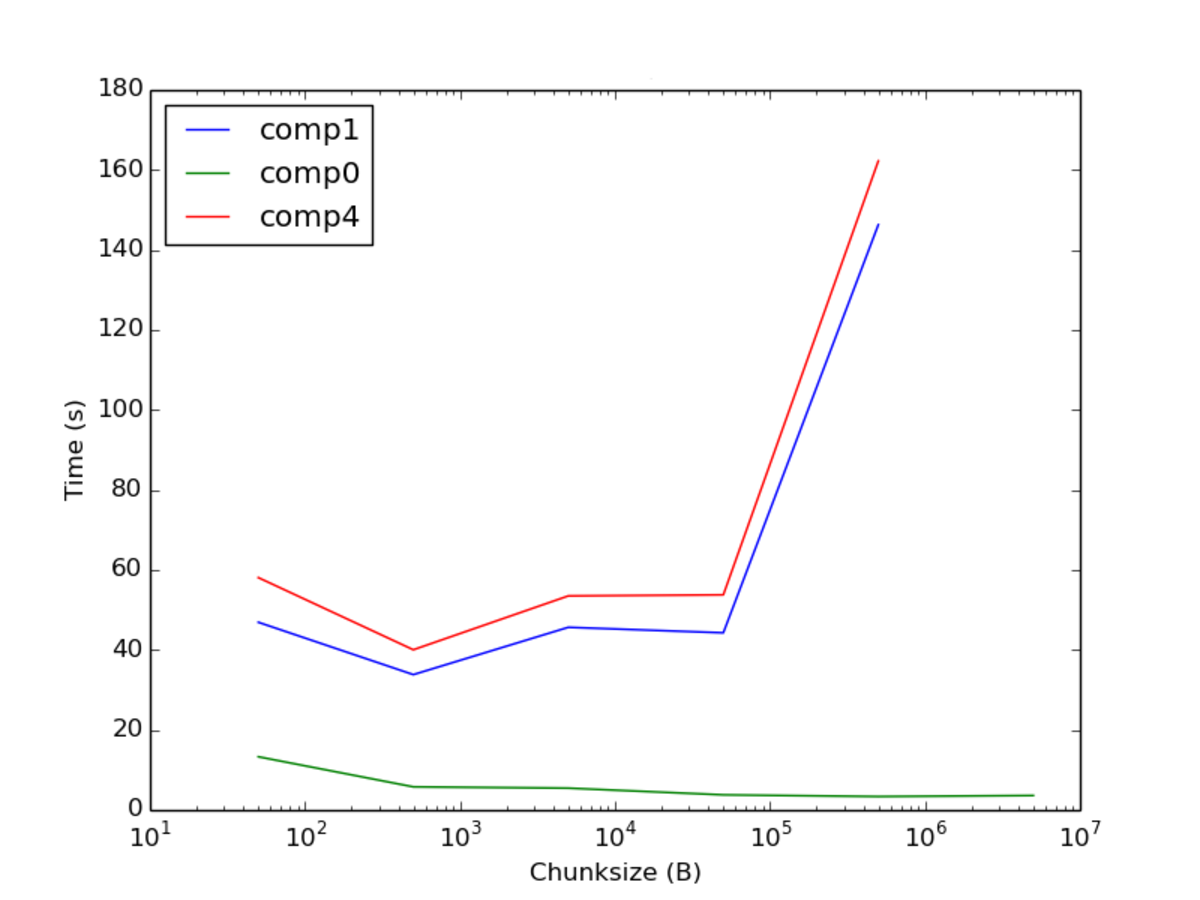
\includegraphics[width=0.85\textwidth]{./backmatter/figs/small_all.pdf}
    \caption{
      \label{fig:small_db}
      Post-processing performance for 25 entries of a small-sized database for a 
      variety of compression levels and chunk sizes.}
  \end{center}
\end{figure}

\begin{figure}
  \begin{center}
    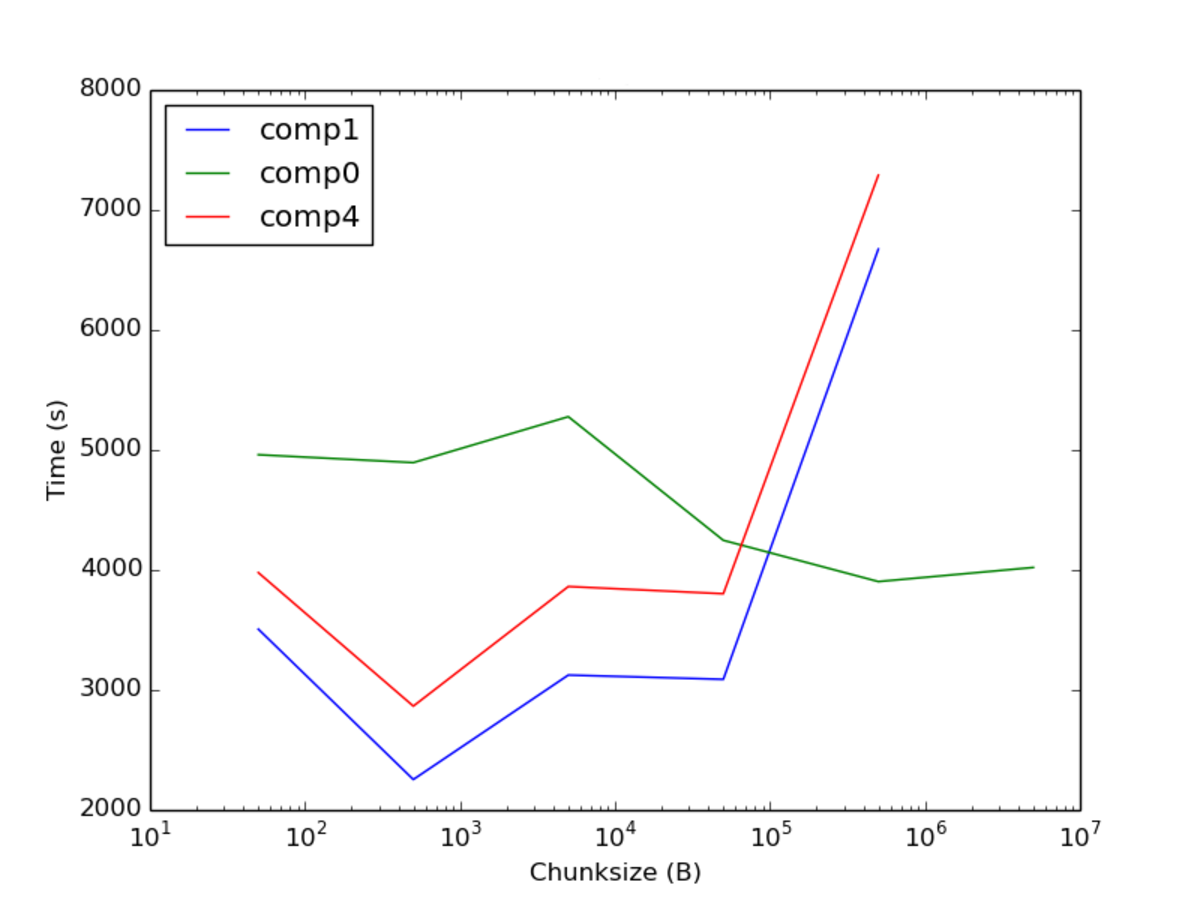
\includegraphics[width=0.85\textwidth]{./backmatter/figs/large_all.pdf}
    \caption{
      \label{fig:large_db}
      Post-processing performance for 25 entries of a large-sized database for a
      variety of compression levels and chunk sizes.}
  \end{center}
\end{figure}

Assuming some level of compression, an ideal chunksize range is identified for
the small database of between $\sim 10^3 - 10^5$ bytes. Further the small
database example confirms that the study's methodology is well founded: an ideal
chunksize range is established. A similar optimal chunk size range is found for
the large database. However, note that in this exercise, only $\sim 0.25\%$ of
instances are post-processed. An optimal performance of $> 80$ seconds per
instance is unacceptable.

A number of strategies exist for trying to increase performance. A classic
strategy is pivoting the group-dataset structure such that data queries are made
upon an entire group rather than rows in a dataset. In this example, such a
pivot involves dividing the single, large dataset into $n$ datasets, where $n$
is the number of unique primary keys, i.e., UUIDs.

Accordingly, an additional performance test was conducted with a new database
layout. All datasets on which queries are made were pivoted such that new group
nodes were added for each UUID, and all data for that UUID was appended to a
dataset under the associated group. The post processing step was divided into
the read and vector-population operations associated with the exchange family
and the the read and vector-population operations associated with a species. The
exact same operations were applied to a large database with the column-based
layout and a large database with the group-based layout. Specific instances,
increasing in size, were identified to be post-processed. The group-based results
were compared with the column-based results and are shown in Figure
\ref{fig:col_grp}. The speed of each operation was compared directly for both
layout strategies. The ratio of the group-strategy running time to the column
strategy running time was then plotted. Therefore, a low ratio implies a large
time savings, and a ratio close to unity implies almost no time savings. Times
were calculated using the IPython magic \texttt{\%timeit} command.

\begin{figure}
  \begin{center}
    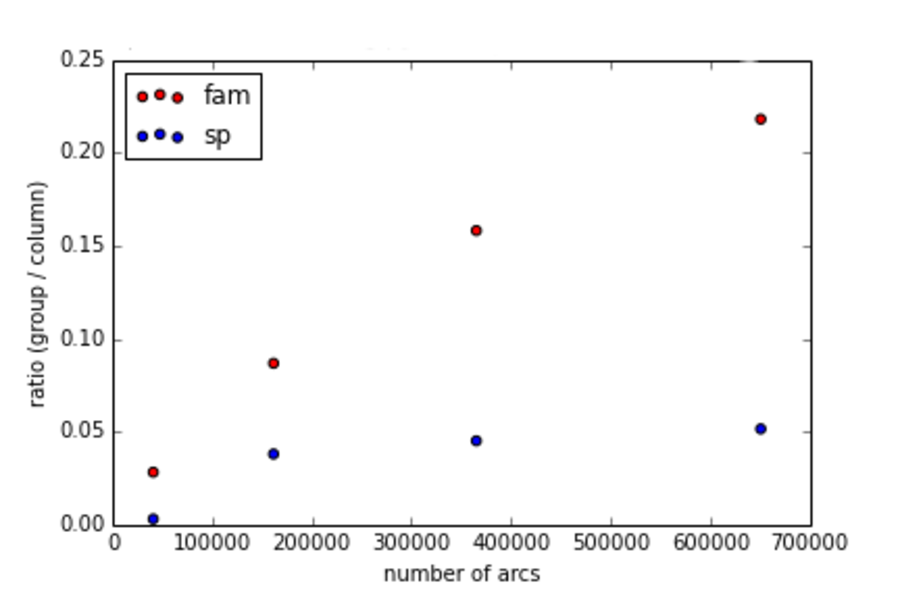
\includegraphics[width=0.85\textwidth]{./backmatter/figs/grp_v_col_ratio.pdf}
    \caption{
      \label{fig:col_grp}
      The ratio of group-based queries to column-based queries as a function of
      problem size. A lower ratio indicates a faster process time for the group
      strategy over the column strategy.}
  \end{center}
\end{figure}

As can be seen, the group-based strategy performs quite well, over an order of
magnitude better than the column-based strategy for species
operations. Furthermore, species operations are shown to have a much larger
speedup relative to family operations. This artifact is due to the fact that at
the time of this analysis, solution values were stored \textit{only if} they
were nonzero. When read, a data structure must be allocated and populated for
each non-zero index rather than simply copying a block on data on disc. The
writing of family-based solution values has since been updated to also write
zero values to avoid this issue.

For the purposes of this study, the dataset-group pivot served the required
purpose. Post-processing now performs satisfactorily for the operations needed
and the database sizes experienced. However, if future performance issues arise,
other strategies may be investigated. Perhaps the most fruitful of these will be
returning to the single dataset layout and using PyTable's indexing feature. 
